%%% Local Variables: 
%%% coding: utf-8
%%% mode: latex
%%% TeX-engine: xetex
%%% End:
\documentclass[12pt,a4paper]{article}
\usepackage[a4paper]{geometry}
\geometry{
 a4paper,
 total={210mm,297mm},
 left=20mm,
 right=25mm,
 top=25mm,
 bottom=20mm,
 }
\usepackage[spanish]{babel}
\def\spanishoptions{argentina}
\usepackage{csquotes}
\usepackage{sparklines}
\usepackage{booktabs}
\usepackage{epigraph}
\usepackage{fontspec}
\defaultfontfeatures{Mapping=tex-text}
\usepackage{xunicode}
\usepackage{graphicx}
\graphicspath{ {images/} }
\usepackage{xltxtra}
\setmainfont{Linux Libertine O}
\usepackage{amsmath}
\usepackage{amsfonts}
\usepackage{amssymb}
\usepackage{url}

\pagestyle{myheadings}

\begin{document}
 \begin{figure}[h!]
   \centering
   
\includegraphics[width=0.20\textwidth]{uba_logo}~\\[1cm]
\title{Hacia una medición sistemática del corte de boleta en Argentina}
\author{
  Universidad de Buenos Aires\\
  Facultad de Ciencias Sociales\\
    Carrera de Ciencia Política \\
    Seminario de Comportamiento Político Electoral - Cátedra Facundo Galván\\
  Franco Mariluis\\
  fmariluis@gmail.com\\
  DNI 29.286.357\\
}
\date{19 de noviembre de 2015}
\maketitle
 \end{figure}

\pagenumbering{gobble}
\clearpage 

\pagenumbering{arabic}
\section{Abstract}
Este trabajo pretende sugerir una metodología concreta para medir el corte de
boleta, que permita la realización de un trabajo comparativo de este
comportamiento aún entre elecciones de
diferentes formas.
Una vez descrita la metodología, intentaremos aplicarla en el caso concreto de
las elecciones provinciales de Chaco 2015, para mostrar si existió alguna
diferencia en el comportamiento electoral de los electores que usaron el sistema
tradicional de papel versus el sistema de Boleta Única Electrónica (en adelante,
BUE). 
En esta elección se dio la particularidad de la convivencia simultánea de ambos
instrumentos de sufragio.\footnote{El autor de
este trabajo se desempeña laboralmente desde el año 2013 como programador en Grupo MSA S.A., que
es la empresa que desarrolla y provee el sistema BUE en varios distritos de Argentina.}

Nos interesa verificar si, en comparación con el sistema tradicional, los
votantes que utilizaron la BUE efectuaron un mayor corte de boleta, debido a la
facilidad que brinda el sistema para \emph{armar} la boleta.


\section{Medición del corte de boleta utilizando la desviación estándar}
La metodología que proponemos para la medición sistemática y comparable es la
siguiente:

Supongamos una elección con tres categorías, por ejemplo, Gobernador, Intendente
y Concejales, y en la que compiten tres partidos, A, B y C, que presentan
candidatos para todos las categorías.

En primer lugar, supongamos que en dicha elección sólo está permitido votar por
lista completa, es decir, no existe la posibilidad de cortar boleta. Un posible
resultado de dicha elección sería el siguiente:

\renewcommand{\arraystretch}{1.25}
\begin{table}[h!]
\centering
\begin{tabular}{c c c c} 
 Partido & Gobernador & Intendente & Concejales \\ [0.5ex] 
 \hline
Partido A & 200 & 200 & 200 \\
Partido B & 100 & 100 & 100 \\
Partido C & 50 & 50 & 50 \\
 \hline
Total & 350 & 350 & 350 \\ [1ex]
 \hline
\end{tabular}
\caption{Elecciones sin corte de boleta habilitado}
\label{table:1}
\end{table}

Ahora bien, supongamos que sí hubiera estado permitido el corte de boleta. En
ese caso, la distribución de votos podría haber sido la siguiente:

\renewcommand{\arraystretch}{1.25}
\begin{table}[h!]
\centering
\begin{tabular}{c c c c} 
 Partido & Gobernador & Intendente & Concejales \\ [0.5ex] 
 \hline
Partido A & 250 & 185 & 50 \\
Partido B & 80 & 100 & 220 \\
Partido C & 20 & 65 & 80 \\
 \hline
Total & 350 & 350 & 350 \\ [1ex]
 \hline
\end{tabular}
\caption{Elecciones con corte de boleta habilitado}
\label{table:1}
\end{table}

Si bien es fácilmente apreciable \emph{a simple vista} la magnitud del corte de boleta, otra cosa es
su medición sistemática. Lo que proponemos para ello es medir la
\emph{desviación estándar} del conjunto de los votos de cada partido, para tener una medida
estandarizada del corte de boleta.

La desviación estándar (también conocida como \(\sigma\)) es una medida de
estadística descriptiva que permite 
cuantificar la dispersión en un grupo de valores. En términos sencillos, indica
qué tanto varían los valores en relación alguna medida de tendencia central como
la media.

Su definición formal es:

\[ \sqrt{\frac{1}{N} \sum_{i=1}^N (x_i - \overline{x})^2} \]

El procedimiento para su cálculo es el siguiente, tomando como ejemplo el
conjunto de valores de votos del Partido A:

\begin{enumerate}
  \item Sumamos todos los votos y los dividimos por 3 para obtener la media:
\[ \frac{250 + 185 + 50}{3} = 161.6666666667\]
  \item A cada valor, le restamos la media obtenida, y  la elevamos al cuadrado,
    dividido por la cantidad de valores. Éste valor es la varianza:
\[\frac{(250 - 166.66)^2 + (185 - 166.66)^2 + (50-166.66)^2}{3} = 6938.8888888889\]
  \item Finalmente, la desviación estandar es la raíz cuadrada de la varianza:
\[\sqrt{6938.8888888889} = 83.2999933307\]
\end{enumerate}

Por ende, según este cálculo, en estas elecciones ficticias el partido A tuvo un
corte de boleta de 83.30 votos (el resultado del cálculo de la desviación
estándar está en la misma unidad que los datos, en este caso, votos).

Probemos ahora de aplicar este cálculo a nuestros dos casos ficticios.

\renewcommand{\arraystretch}{1.25}
\begin{table}[h!]
\centering
\begin{tabular}{c c c c c} 
 Partido & Gobernador & Intendente & Concejales & \(\sigma\) \\ [0.5ex] 
 \hline
Partido A & 200 & 200 & 200 & 0 \\
Partido B & 100 & 100 & 100 & 0 \\
Partido C & 50 & 50 & 50 & 0 \\
 \hline
Total & 350 & 350 & 350 & 0 \\ [1ex]
 \hline
\end{tabular}
\caption{Elecciones sin corte de boleta habilitado, con cálculo de \(\sigma\)}
\label{table:1}
\end{table}

\pagebreak

Aplicando el cálculo de $\sigma$ al caso donde no es posible el corte de boleta,
obtenemos el resultado esperado de 0 votos de corte. Veamos qué sucede en el
caso siguiente:

\renewcommand{\arraystretch}{1.25}
\begin{table}[h!]
\centering
\begin{tabular}{c c c c c} 
 Partido & Gobernador & Intendente & Concejales & $\sigma$ \\ [0.5ex] 
 \hline
Partido A & 250 & 185 & 50 & 83.30 \\
Partido B & 80 & 100 & 220 & 61.82 \\
Partido C & 20 & 65 & 80 & 25.49 \\
 \hline
Total & 350 & 350 & 350 & 56.87 (promedio) \\ [1ex]
 \hline
\end{tabular}
\caption{Elecciones con corte de boleta habilitado, con cálculo de $\sigma$}
\label{table:1}
\end{table}

Apliquemos esta metodología a un ejemplo real, en un caso donde sabemos que se verificó
ciertamente un alto grado de corte de boleta: el municipio de Lanús, en las
elecciones generales 2015. En este partido, ganó el Frente para la Victoria para
la categoría de Presidente y Cambiemos para Gobernador e Intendente.

\renewcommand{\arraystretch}{1.25}
\begin{table}[h!]
\centering
\begin{tabular}{c c c c c c} 
 Partido & Presidente & Gobernador & Intendente & $\sigma$ & $\sigma$ como \% de votos \\ [0.5ex] 
 \toprule
FPV & 107297 & 95815 & 99430 & 4793.45 & 4.75\% \begin{sparkline}{10}
\sparkdot 0.1 1 blue
\sparkdot 0.5 0.3 red
\spark 0.1 1  0.5 0.3  1 0.7 /
\end{sparkline}
\\
Cambiemos & 96588 & 113067 & 103362 & 6762.90 & 6.48\% \begin{sparkline}{10}
\sparkdot 0.5 1 blue
\sparkdot 0.1 0.5 red
\spark 0.1 0.5  0.5 1  1 0.8 /
\end{sparkline}
\\
UNA & 61727 & 51614 & 54669 & 4235.05 & 7.56\% \begin{sparkline}{10}
\sparkdot 0.1 0.7 blue
\sparkdot 0.5 0.25 red
\spark 0.1 0.7  0.5 0.25  1 0.40 /
\end{sparkline}
\\
FIT & 11979 & 11901 & 11462 & 227.57 & 1.93\% \begin{sparkline}{10}
\sparkdot 0.1 0.55 blue
\sparkdot 0.5 0.50 red
\spark 0.1 0.55  0.5 0.50  1 0.40 /
\end{sparkline}
\\
Progresistas & 8634 & 6653 & 6568 & 954.52 & 13.10\% \begin{sparkline}{9}
\sparkdot 0.1 0.8 blue
\sparkdot 1 0.20 red
\spark 0.1 0.8  0.5 0.25  1 0.20 /
\end{sparkline}
\\
 \hline
\end{tabular}
\caption{Elecciones Generales en Lanús, 2015}
\label{table:1}
\end{table}

De esta tabla\footnote{La última columna del cuadro 5 muestra la desviación
  estándar como porcentaje del total de votos del partido. La visualización es
  una \emph{sparkline}, y permite ver cómo se deslizó el corte de boleta en cada
partido. Sobre \emph{sparklines}, ver
\url{https://www.edwardtufte.com/bboard/q-and-a-fetch-msg?msg_id=0001OR}}
podemos desprender ya algunos elementos de análisis, sobre todo si
expresamos la desviación estándar en términos porcentuales sobre el total de
votos obtenido por cada partido.
\begin{enumerate}
  \item FIT tiene un corte de boleta bajísimo, al parecer señal de que sus votantes votan más al partido
    que a las opciones particulares de cada categoría
  \item Progresistas tiene el corte de boleta más alto, sobre todo
    en la categoría Presidente. Probablemente porque su candidata a Presidente
    es la figura más conocida el partido.
  \item El corte de boleta del FPV no es tan alto, pero combinado con el corte
    que registra Cambiemos y UNA, se explica el resultado disímil que obtuvo
    para Presidente y Gobernador.
\end{enumerate}

Algunas condiciones son fundamentales para poder utilizar correctamente esta
metodología:

\begin{itemize}
  \item Debemos contar solamente los partidos que presenten candidatos a todas
    las categorías, de otro modo se produciría una distorsión en la medida.
  \item La desviación estándar se cuenta de modo horizontal, en una matriz donde
    las columnas son cargos y las filas son partidos.
  \item Es necesario contar empezando desde el nivel más bajo posible,
    idealmente mesa, a fin de tener todas las categorías contempladas desde su
    primer nivel significativo.
\end{itemize}

\pagebreak

\section{Estudio de caso: las elecciones chaqueñas de 2015}

En esta parte haremos una aplicación práctica de esta metodología para comparar
el comportamiento electoral de los votantes chaqueños durante las elecciones
provinciales del 20 de septiembre de 2015, teniendo en cuenta que en dichas
elecciones convivieron dos instrumentos de sufragio: el sistema tradicional de
boletas de papel y el sistema de Boleta Única Electrónica. Éste último se aplicó
en el 100\% de las mesas de la localidad de Resistencia, y en algunas mesas del
interior de la provincia.

Nos interesa verificar si existieron diferencias en el corte de boleta entre
ambos sistemas, dado que se supone que la BUE facilita esta tarea al elector, al
permitirle construir su opción electoral en una pantalla y realizar los cambios
necesarios antes de la impresión de la boleta.

\subsection{La Boleta Única Electrónica}
La Boleta Única Electrónica es un sistema de sufragio que permite que elector
realice la selección de sus candidatos en una pantalla táctil, para luego
confirmar su elección e imprimir una boleta (la cual posee la información
grabada en un chip). Ésta boleta se deposita en una urna tradicional y es
recontada al cierre de mesas.

En relación al aspecto que nos interesa analizar, la interfaz gráfica de la
máquina de voto hace más sencillo al votante elegir a los candidatos para cada
categoría (en comparación al sistema tradicional, que implica cortar físicamente
varias boletas de papel).

Si bien permite también la seleccion \emph{por lista completa}, la interfaz
elimina la fricción inherente al acto de elegir distintos partidos para cada
categoría, y por ende debería reflejarse en un mayor corte de boleta medido con
los resultados.

\begin{figure}[h]
\centering
    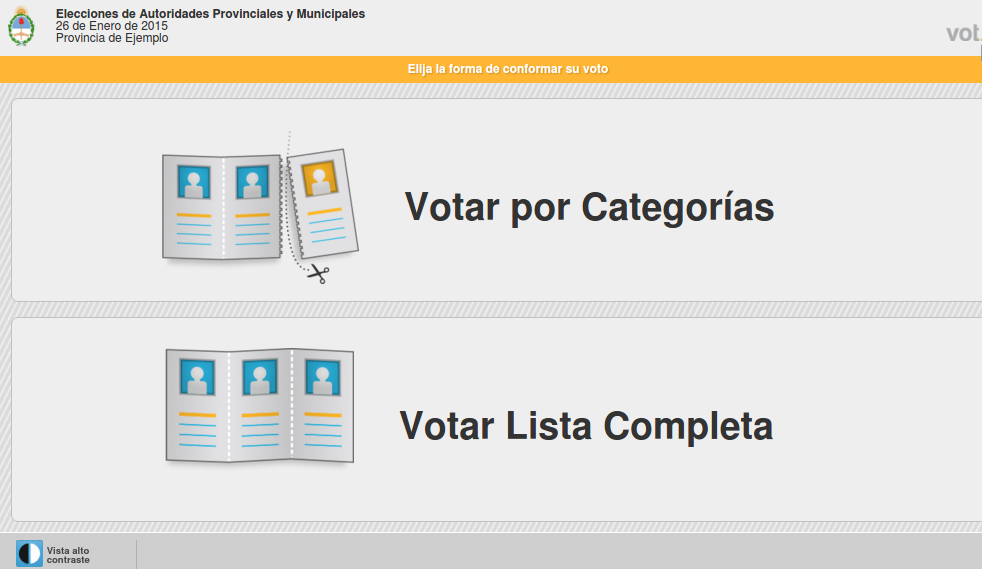
\includegraphics[width=\textwidth]{interfaz_bue}
\caption{Interfaz del sistema BUE}
\end{figure}

\subsection{Análisis de las elecciones 2015}

\renewcommand{\arraystretch}{1.25}
\begin{table}[h!]
\centering
\begin{tabular}{c c c c} 
 Departamento & Electores & Mesas Tradicionales & Mesas Electrónicas \\ [0.5ex] 
 \hline
SAN FERNANDO & 320273 & 290 & 804 \\
PRIMERO DE MAYO &	9705 & 41 & 0 \\
LIBERTAD & 9906 & 42 & 0 \\
GRAL.DONOVAN & 11829 & 46 & 0 \\
SARGENTO CABRAL &	14092 & 53 & 0 \\
PCIA. DE LA PLAZA &	9512 & 36 & 0 \\
BERMEJO	& 21975 & 88 & 0 \\
LIB.GRAL.SAN MARTIN	& 47381 & 172 & 0 \\
TAPENAGA & 2962 & 16 & 0 \\
SAN LORENZO &	12373 & 44 & 100 \\
MAYOR L.J.FONTANA &	45522 & 128 & 31 \\
O HIGGINS	& 16624 & 61 & 0 \\
COMANDANTE FERNANDEZ & 74956 & 249 & 9 \\
QUITILIPI	& 27092 & 94 & 0 \\
25 DE MAYO & 23224 & 84 & 0 \\
MAIPU & 19545 & 67 & 0 \\
INDEPENDENCIA	& 17123 & 64 & 0 \\
GENERAL BELGRANO & 9207 & 34 & 0 \\
9 DE JULIO & 22575 & 78 & 0 \\
CHACABUCO	& 25100 & 56 & 30 \\
12 DE OCTUBRE &	18368 & 65 & 0 \\
2 DE ABRIL & 5643 & 21 & 0 \\
FRAY J.STA.MARIA DE ORO	& 9739 & 34 & 0 \\
ALMIRANTE BROWN	& 26578 & 95 & 0 \\
GENERAL GUEMES & 57857 & 201 & 0 \\ 
 \hline
Total & 859161 & 2159 & 874 \\ [1ex]
 \hline
\end{tabular}
\caption{Electores y tipos de mesas - Chaco 2015}
\label{table:1}
\end{table}

El cuadro 6 muestra la distribución de mesas según tipo de instrumento de
sufragio habilitado. De un total de 856.161 electores habilitados, un total de
256.521 (casi un 30\%) votaron con BUE.

Siguiendo con las recomendaciones de la sección anterior, de todo el espectro de
partidos participantes sólo vamos a tomar para este análisis a los tres partidos
que presentaron candidato a Gobernador:

\begin{itemize}
  \item Frente Chaco Merece Más
  \item Vamos Chaco
  \item Partido del Obrero
\end{itemize}

Además, y para trabajar con un conjunto de datos más homogéneo, vamos a eliminar
las mesas que poseen menos de 100 electores habilitados (87 mesas).

Veamos una primera aproximación al cálculo de la desviación estándar por partido
de este conjunto de datos, dividido según mesas electrónicas y tradicionales:

\begin{table}[h!]
\centering
\label{my-label}
\begin{tabular}{c c c}
 & Electrónicas & Tradicionales \\
\hline
Mínimo & 0.00 & 0.00 \\
1er. cuartil & 2.165 & 1.00 \\
Mediana & 3.031 & 2.121 \\
Promedio & 3.269 & 3.581 \\
3er. cuartil & 4.153 & 4.387 \\
Máximo & 11.820 & 58.270 \\
\hline
\end{tabular}
\caption{Estadística descriptiva: sigmas de cortes de boleta}
\label{table:1}
\end{table}

Llama la atención el valor máximo de la desviación estándar de las mesas
tradicionales, lo que parece indicar que existen valores muy elevados en el 3er
cuartil. Eso explica por qué el promedio de corte de boleta es más alto en el
conjunto tradicional que en el electrónico, aunque la mediana sea más alta en
éste último.

Veamos la dispersión de valores del sistema tradicional en un histograma:

\begin{figure}[h]
\centering
    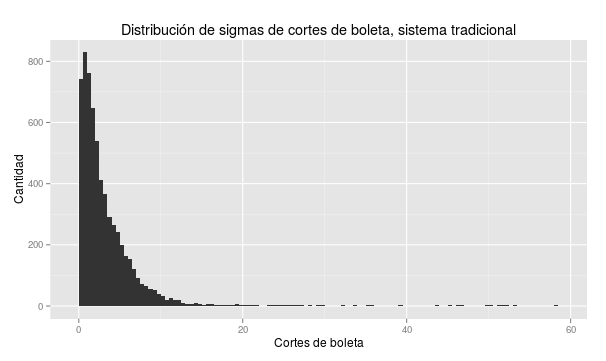
\includegraphics[width=\textwidth]{sigmas_tradicional}
\caption{Histograma de cortes de boleta, sistema tradicional}
\end{figure}

Es evidente que existen anomalías en el conjunto de datos: podemos como existen
valores muy altos (desviación estándar de más de 17 votos) pero de poca
ocurrencia. Estadísticamente, estamos muy lejos de una distribución normal.

Veamos la dispersión en los valores del sistema BUE:

\begin{figure}[h]
\centering
    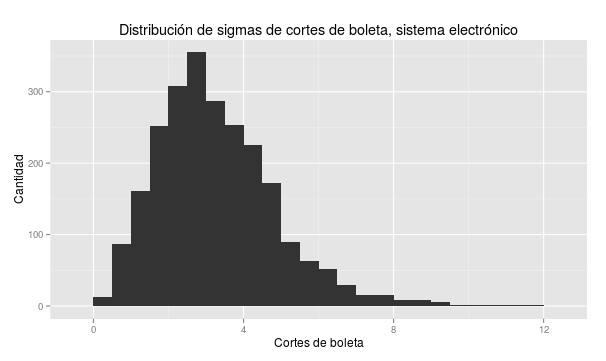
\includegraphics[width=\textwidth]{sigmas_electronico}
\caption{Histograma de cortes de boleta, sistema electrónico}
\end{figure}

Aquí vemos una distribución de valores mucho más normal. Si nos enfocamos
puntualmente en los valores altos, detectamos que se concentran mayormente en
algunas localidades donde los votos del Frente Chaco Merece Más para intendente
fueron a favorecer al candidato de un partido local sin candidatos a Gobernador.
Vemos entonces que la aplicación de esta metodología se aplica también a la
detección de este tipo de casos que pueden constituir una anomalía.

Volviendo al conjunto de datos tradicional, las mesas que cuentan con
un sigma mayor a 20 en toda la provincia son 221 (7.28\% del total), de las
cuales un número muy alto (77) se concentran en un mismo municipio (Villa Rio
Bermejito), donde para las categorías locales de Intendente y Concejales triunfó
ampliamente un partido local. Este hecho cambia el peso en la distribución de
valores, haciendo que pocos valores pero muy altos cambien la tendencia central.

A efectos de nuestro análisis comparativo, descartemos esa porción de mesas y
verifiquemos nuevamente la distribución de valores:

\begin{table}[h!]
\centering
\label{my-label}
\begin{tabular}{c c c}
 & Electrónicas & Tradicionales (sigma < 12) \\
\hline
Mínimo & 0.00 & 0.00 \\
1er. cuartil & 2.165 & 0.866 \\
Mediana & 3.031 & 2.046 \\
Promedio & 3.269 & 2.793 \\
3er. cuartil & 4.153 & 4.085 \\
Máximo & 11.820 & 11.950 \\
\hline
\end{tabular}
\caption{Estadística descriptiva: sigmas de cortes de boleta (tradicional con
  sigma < 12)}
\label{table:1}
\end{table}

Y si graficamos nuevamente la distribución:

\begin{figure}[h]
\centering
    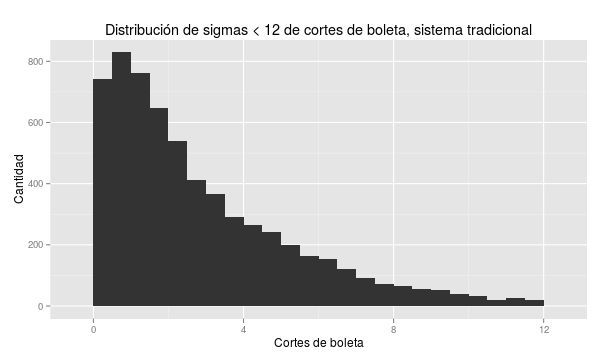
\includegraphics[width=\textwidth]{sigmas_tradicional_menor_a_12}
\caption{Histograma de cortes de boleta, sistema tradicional con sigmas menores
  a 12}
\end{figure}

Vemos aquí con claridad, tanto en el gráfico como en la estadística descriptiva,
que en las mesas electrónicas se da una mayor frecuencia de valores altos de
cortes de boleta, lo que parece reforzar nuestra hipótesis inicial.

\section{Conclusiones}
En este trabajo intentamos describir una metodología para medir de manera
sistemática el corte de boleta electoral, y permitir la realización de análisis
comparativos aún tratándose de elecciones diferentes.

Creemos que al estar basado en una medida estadística descriptiva reconocida
como la desviación estándar, esta metodología puede ser aplicable con relativa
sencillez, salvando la dificultad (por otro lado habitual en cualquier
investigación que trabaje con datos) de reorganizar el conjunto de datos de
origen para que tenga la forma sugerida.

Una vez presentada la metodología, pudimos aplicarla a un caso electoral
concreto a fin de mostrar diferencias en el comportamiento electoral de los
votantes según el instrumento de sufragio: vimos que, siendo en la misma
elección, el corte de boleta es sensiblemente mayor en el caso de la Boleta
Única Electrónica que en el sistema tradicional.

Sería interesante en futuras investigaciones la exploración de otras hipótesis.

\pagebreak

\section{Bibliografía y Fuentes}

\begin{itemize}
  \item Galván, Facundo (2014). “¿Hacia dónde va el voto electrónico?”, columna publicada en el sitio web de noticias www.NoticiasElectorales.com Disponible en: http://www.noticiaselectorales.com/argentina-hacia-donde-va-el-voto-electronico
  \item Datos de elecciones provinciales de Chaco 2015 disponibles en \url{http://elecciones2015.electoralchaco.gov.ar/}
  \item Datos de elecciones en el partido de Lanús tomadas de
    \url{http://www.elecciones.gov.ar/articulo_sub_sub.php?secc=2&sub_secc=55&sub_sub_secc=64}
    y \url{http://www.resultadosba.gob.ar/resultados/dat02/DCO02062M.htm?d=1543}
  \item Este trabajo fue escrito utilizando \LaTeX. Los cálculos estadísticos y
    gráficos fueron generados en R.
  \item Tablas utilizadas, datos base y código fuente del trabajo disponibles en \url{https://github.com/fmariluis/paper-cortedeboleta}
\end{itemize}

\tableofcontents
\listoftables
\listoffigures

\end{document}
